\hypertarget{what-is-javascript}{%
\chapter{JavaScript\index{JavaScript}とは}\label{what-is-javascript}}
\thispagestyle{frontheadings}

JavaScriptを学びはじめる前に、まずJavaScriptとはどのようなプログラミング言語なのかを紹介します。

JavaScriptは主にウェブブラウザの中で動くプログラミング言語です。
ウェブサイトで操作をしたら表示が書き換わったり、ウェブサイトのサーバーと通信してデータを取得したりと現在のウェブサイトには欠かせないプログラミング言語です。
このようなJavaScriptを活用してアプリケーションのように操作できるウェブサイトをウェブアプリとも言います。

JavaScriptはウェブブラウザだけではなく、Node.jsというサーバー側のアプリケーションを作る仕組みでも利用されています。
また、デスクトップアプリやスマートフォンアプリ、IoT(Internet of Things)デバイスでもJavaScriptを使って動かせるものがあります。
このように、JavaScriptはかなり幅広い環境で動いているプログラミング言語で、さまざまな種類のアプリケーションを作成できます。

\hypertarget{javascript-ecmascript}{%
\section{JavaScriptとECMAScript\index{ECMAScript}}\label{javascript-ecmascript}}

JavaScriptという言語は\hyperlink{ecmascript}{ECMAScript}という仕様によって動作が決められています。
\hyperlink{ecmascript}{ECMAScript}という仕様では、どの実行環境でも共通な動作のみが定義されているため、基本的にどの実行環境でも同じ動作をします。

一方で、実行環境によって異なる部分もあります。
たとえば、ブラウザではUI(ユーザーインターフェース)を操作するためのJavaScriptの機能が定義されていますが、サーバー側の処理を書くNode.jsではそれらの機能は不要です。
このように、実行環境によって必要な機能は異なるため、それらの機能は実行環境ごとに定義(実装)されています。

そのため、「ECMAScript」はどの実行環境でも共通の部分、「JavaScript」はECMAScriptと実行環境の固有機能も含んだ範囲というのがイメージしやすいでしょう。

\begin{figure}
\centering
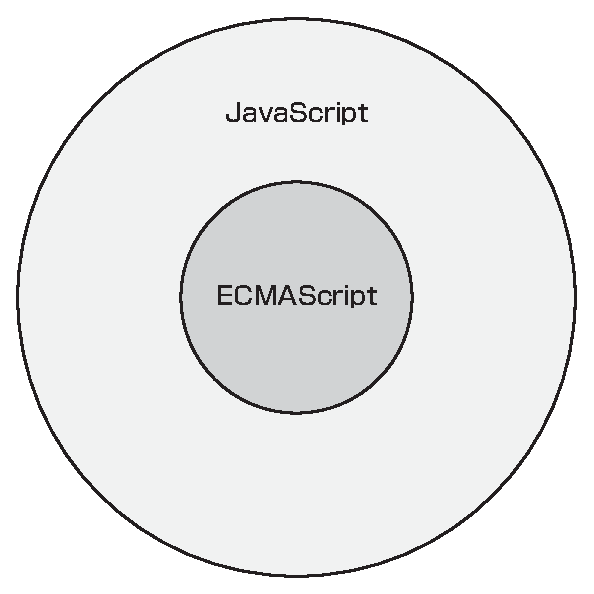
\includegraphics[width=60mm]{./fig/javascript-ecmascript.eps}
\caption{JavaScriptとECMAScriptの範囲}
\end{figure}

ECMAScriptの仕様で定義されている機能を学ぶことで、どの実行環境でも対応できる基本的な部分を学べます。
この書籍では、この違いを明確に区別する必要がある場合は「ECMAScript」と「JavaScript」という単語を使い分けます。
そうでない場合、「JavaScript」という単語を使います。

また、このECMAScriptという仕様(共通の部分)も毎年アップデートされ、新しい文法や機能が追加されています。
そのため、実行環境によっては古いバージョンのECMAScriptを実装したものとなっている場合があります。
ECMAScriptは2015年にECMAScript 2015\index{ECMAScript 2015}(ES2015\index{ES2015})として大きくアップデートされた仕様が公開されました。

今からJavaScriptを学ぶなら、ES2015以降を基本にしたほうがわかりやすいため、この書籍はES2015に基づいた内容となっています。
また、既存のコードはES2015より前のバージョンを元にしたものも多いため、それらのコードに関しても解説しています。

まずは、JavaScript(ECMAScript)とはどのような言語なのかを大まかに見ていきます。

\hypertarget{about-javascript}{%
\section{JavaScriptってどのような言語?}\label{about-javascript}}

JavaScriptは、元々Netscape Navigatorというブラウザのために開発されたプログラミング言語です。
C、Java、Self、Schemeなどのプログラミング言語の影響を受けて作られました。

JavaScriptは、大部分がオブジェクト(値や処理を1つにまとめたものと考えてください)であり、そのオブジェクト同士のコミュニケーションによって成り立っています。
オブジェクトには、ECMAScriptの仕様として定められたオブジェクト、
実行環境が定義したオブジェクト、ユーザー(つまりあなたです)の定義したオブジェクトが存在します。

この書籍の「\hyperlink{basic-grammar}{第1部 基本文法}」ではECMAScriptの定義する構文やオブジェクトを学んでいきます。
「\hyperlink{use-case}{第2部 ユースケース}」ではブラウザやNode.jsといった実行環境が定義するオブジェクトを学びながら、小さなアプリケーションを作成していきます。
ユーザーの定義したオブジェクトは、コードを書いていくと自然と登場するため、適宜見ていきます。

次に、JavaScriptの言語的な特徴を簡単に紹介していきます。

\hypertarget{case-sensitive}{%
\subsection{大文字と小文字を区別する}\label{case-sensitive}}

まず、JavaScriptは大文字小文字を区別します。
たとえば、次のように\texttt{name}という変数を大文字と小文字で書いた場合に、
それぞれは別々の\texttt{name}と\texttt{NAME}という名前の変数として認識されます。

\begin{lstlisting}
// nameという名前の変数を宣言
const name = "azu";
// NAMEという名前の変数を宣言
const NAME = "azu";
\end{lstlisting}

また、大文字で開始しなければならないといった命名規則が意味を持つケースはありません。
そのため、あくまで別々の名前として認識されるというだけになっています
(変数についての詳細は「\hyperlink{variable-and-declaration}{変数と宣言}」の章で解説します)。

\hypertarget{reserved-keyword}{%
\subsection{予約語\index{よやくご@予約語}を持つ}\label{reserved-keyword}}

JavaScriptには特別な意味を持つキーワードがあり、これらは予約語とも呼ばれます。
このキーワードと同じ名前の変数や関数は宣言できません。
先ほどの、変数を宣言する\texttt{const}も予約語のひとつとなっています。
そのため、\texttt{const}という名前の変数名は宣言できません。

\hypertarget{statement-semicolon}{%
\subsection{文\index{ぶん@文}はセミコロン\index{せみころん@セミコロン}で区切られる}\label{statement-semicolon}}

JavaScriptは、文(Statement\index{Statement})ごとに処理していき、文はセミコロン(\texttt{;}\index{;@\texttt{;}})によって区切られます。
特殊なルールに基づき、セミコロンがない文も、行末に自動でセミコロンが挿入されるという仕組みも持っています\footnote{Automatic Semicolon Insertion\index{Automatic Semicolon Insertion}と呼ばれる仕組みです。}。
しかし、暗黙的なものへ頼ると意図しない挙動が発生するため、セミコロンは常に書くようにします
(詳細は「\hyperlink{statement-and-expression}{文と式}」の章で解説します)。

また、スペース、タブ文字などは空白文字\index{くうはくもじ@空白文字}(ホワイトスペース\index{ほわいとすぺーす@ホワイトスペース})と呼ばれます。
これらの空白文字を文にいくつ置いても挙動に違いはありません。

たとえば、次の\texttt{1}足す\texttt{1}を行う2つの文は、\texttt{+}の前後の空白文字の個数に違いはありますが、動作としてはまったく同じ意味となります。

\begin{lstlisting}
// 式や文の間にスペースがいくつあっても同じ意味となる
1 + 1;
1   +   1;
\end{lstlisting}

空白文字の置き方は人によって好みが異なるため、人によって書き方が異なる場合もあります。
複数人で開発する場合は、これらの空白文字の置き方を決めたコーディングスタイル\index{こーでぃんぐすたいる@コーディングスタイル}を決めるとよいでしょう。
コーディングスタイルの統一については「\hyperlink{reference-links}{付録A 参考リンク集}」を参照してください。

\hypertarget{strict-mode}{%
\subsection{strict mode\index{strict mode}}\label{strict-mode}}

JavaScriptには\textbf{strict mode}という実行モードが存在しています。
名前のとおり厳格な実行モードで、古く安全でない構文や機能が一部禁止されています。

\texttt{"use strict"}という文字列をファイルまたは関数の先頭に書くことで、そのスコープにあるコードはstrict modeで実行されます。
また、後述する"Module"の実行コンテキストでは、このstrict modeがデフォルトとなっています。\enlargethispage{\baselineskip}

\begin{lstlisting}
"use strict";
// このコードはstrict modeで実行される
\end{lstlisting}

strict modeでは、\texttt{eval}や\texttt{with}といったレガシーな機能や構文を禁止します。
また、明らかな問題を含んだコードに対しては早期的に例外を投げることで、開発者が間違いに気づきやすくしてくれます。

たとえば、次のような\texttt{const}などのキーワードを含まずに変数を宣言しようとした場合に、strict modeでは例外が発生します。
strict modeでない場合は、例外が発生せずにグローバル変数が作られます。

\begin{lstlisting}
"use strict";
mistypedVariable = 42; // => ReferenceError
\end{lstlisting}

このように、strict modeでは開発者が安全にコードを書けるように、JavaScriptの落とし穴を一部ふさいでくれます。
そのため、常にstrict modeで実行できるコードを書くことが、より安全なコードにつながります。

本書では、明示的に「strict modeではない」ことを宣言した場合を除き、
すべてstrict modeとして実行できるコードを扱います。

\hypertarget{script-module}{%
\subsection{実行コンテキスト\index{じっこうこんてきすと@実行コンテキスト}: Script\index{Script}とModule\index{Module}}\label{script-module}}

JavaScriptの実行コンテキストとして"Script"と"Module"があります。
コードを書く場合には、この2つの実行コンテキストの違いを意識することは多くありません。

"Script"の実行コンテキストは、多くの実行環境ではデフォルトの実行コンテキストです。
"Script"の実行コンテキストでは、デフォルトはstrict modeではありません。

"Module"の実行コンテキストは、JavaScriptをモジュールとして実行するために、ECMAScript 2015で導入されたものです。
"Module"の実行コンテキストでは、デフォルトがstrict modeとなり、古く安全でない構文や機能は一部禁止されています。
また、モジュールの機能は"Module"の実行コンテキストでしか利用できません。モジュールについての詳細は「\hyperlink{module}{ECMAScriptモジュール}」の章で解説します。

\hypertarget{ecmascript-updates}{%
\subsection{JavaScriptの仕様は毎年更新される}\label{ecmascript-updates}}

最後に、JavaScriptの仕様であるECMAScriptは毎年更新され、JavaScriptには新しい構文や機能が増え続けています。
そのため、この書籍で学んだ後もまだまだ知らなかったことが出てくるはずです。

一方で、ECMAScriptは後方互換性が慎重に考慮されているため、過去に書いたJavaScriptのコードが動かなくなる変更はほとんど入りません。
そのため、この書籍で学んだことのすべてが無駄になることはありません。

ECMAScriptの仕様がどのように策定されているかについては「\hyperlink{ecmascript}{ECMAScript}」の章で解説します。
